\chapter{บทนำ}
\label{chapter:introduction}

\section{การเขียนรายงาน}

นักศึกษาจะต้องเขียนรายงานให้ถูกต้องตามรูปแบบที่กำหนด นอกเหนือจากรูปแบบของรายงานแล้ว นักศึกษาควรให้ความสำคัญกับการใช้ภาษาและการจัดเรียงหัวข้อที่ต่อเนื่อง รวมถึงการอธิบายที่กระชับแต่ได้ใจความ อันเป็นลักษณะของการเขียนรายงานทางวิชาการที่ดี คำศัพท์ต่าง ๆ ต้องเขียนให้ถูกตามศัพท์บัญญัติราชบัณฑิตยสถาน ซึ่งสามารถตรวจสอบได้ที่ \url{http://www.royin.go.th/?page_id=15521}

หากมีการอ้างอิงข้อมูลจากแหล่งอื่นๆ นักศึกษาสามารถทำได้โดยมี 2 วิธี ดังนี้
\begin{enumerate}
    \item ต้องเขียนด้วยสำนวนของตนเอง และอ้างอิงถึงแหล่งที่มาของความคิดนั้นๆ
    \item ถ้าคัดลอกข้อความใดๆ มาจะต้องทำการอ้างอิงพร้อมใส่เครื่องหมายอัญประกาศคร่อมประโยคนั้นๆอนึ่งการคัดลอกวิธีนี้สามารถทำได้โดยไม่เกิน 15\% ของจำนวนข้อความทั้งหมดของเล่มรายงาน
\end{enumerate}

\textbf{หมายเหตุ ถ้ากรรมการตรวจพบการคัดลอกโดยไม่ตรงตามข้อกำหนด นักศึกษาจะถูกทำโทษโดยการได้รับผลคะแนนเป็น F ทันที}

\section{รูปแบบรายงาน}
\subsection{ส่วนประกอบของรายงานและการเรียงลำดับ}
\begin{itemize}
    \item \textbf{ปกนอก} (ภาษาไทย) ให้ใช้กระดาษขาวลักษณะเดียวกับที่ใช้พิมพ์ตัวรายงานเป็นปกนอก พร้อมพิมพ์ชื่อเรื่อง ชื่อนักศึกษา ชื่ออาจารย์ที่ปรึกษา รหัสประจำตัว และชื่อวิชา (ไม่ต้องใส่คำนำหน้าชื่อ อาจารย์ที่ปรึกษาใช้ตัวอักษรขนาด 20 ตัวหนา ส่วนล่างตั้งแต่ ``ปริญญานิพนธ์นี้... ''ใช้ตัวอักษรขนาด 18 ตัวหนา) ดูตัวอย่างในภาคผนวก
    \item \textbf{ปกใน} (ภาษาอังกฤษ) ใช้ตัวพิมพ์ใหญ่ทั้งหมด โดยมีขนาด 20 ตัวหนา ส่วนล่างตั้งแต่ ``A PROJECT SUBMITTED IN PARTIAL... '' ใช้ตัวอักษรขนาด 18 ตัวหนา
    \item \textbf{Copyright} อยู่ส่วนล่างของหน้ากระดาษด้านซ้าย ใช้ตัวอักษรขนาด 18ตัวหนา (แสดงปีที่ตีพิมพ์ปัจจุบัน)
    \item \textbf{ใบรับรองปริญญานิพนธ์} ตั้งแต่คำว่า ใบรับรองปริญญานิพนธ์... จนถึงสถาบันฯ (3 บรรทัดแรก) ใช้ขนาดอักษร 24 ตัวหนา ส่วนคำว่า เรื่อง ภาษาไทยและภาษาอังกฤษ (ตัวอักษรพิมพ์ใหญ่) และผู้จัดทำ ขนาดตัวอักษร 20 หนา ชื่ออาจารย์ที่ปรึกษาและที่ปรึกษาร่วม (ถ้ามี) ขนาดอักษร 18 หนา
    \item \textbf{ใบรับรองโครงงาน} (เฉพาะรายงานต้นฉบับและรายงานฉบับสมบูรณ์) ใบรับรองการตรวจสอบและอนุมัติรายงาน ตั้งแต่คำว่า ``ใบรับรองโครงงาน... '' จนถึงรหัสประจำตัว ใช้ตัวอักษรขนาด 20 ตัวหนาในส่วนของคำว่า ``ขอรับรองว่า... '' ใช้ตัวอักษรขนาด 16 ตัวหนา และในส่วนของคำว่า ``อาจารย์ที่ปรึกษา/กรรมการ.. '' ใช้ตัวอักษรขนาด 16 ตัวหนา
    \item \textbf{บทคัดย่อภาษาไทย} ประกอบด้วยชื่อหัวข้อโครงงาน ชื่อนักศึกษา ชื่ออาจารย์ที่ปรึกษา ระดับการศึกษา และปีการศึกษา ดังตัวอย่างในภาคผนวก (คำว่า ``บทคัดย่อ'' ใช้ตัวอักษรขนาด 24 ตัวหนา)
    \item \textbf{บทคัดย่อภาษาอังกฤษ} มีรูปแบบเช่นเดียวกับบทคัดย่อภาษาไทยดังตัวอย่างในภาคผนวก (คำว่า ``ABSTRACT'' ใช้ ตัวอักษรขนาด 24ตัวหนา)
    \item \textbf{กิตติกรรมประกาศ} ใช้กล่าวขอบคุณบุคคลที่มีส่วนช่วยเหลือในการศึกษา (คำว่า ``กิตติกรรมประกาศ'' ใช้ตัวอักษรขนาด 24 ตัวหนา)
    \item \textbf{สารบัญ} ซึ่งแสดงเลขที่หน้าของ บทคัดย่อ สารบัญ กิตติกรรมประกาศ บทต่างๆ ในส่วนของเนื้อหา บรรณานุกรม ฯลฯ มีคำว่า ``สารบัญ'' ตรงกลางหน้าใช้ตัวอักษรขนาด 24 ตัวหนาถ้ามีต่อหน้า 2 มีคำว่า ``สารบัญ (ต่อ)
    \item \textbf{สารบัญรูป/สารบัญตาราง} อาจมีหรือไม่ก็ได้ขึ้นอยู่กับเนื้อหาภายในเล่ม ถ้ามีจะอยู่ถัดจากหน้าสารบัญ คำว่า ``สารบัญรูป'' ใช้ตัวอักษรขนาด 24 ตัวหนาถ้ามีต่อหน้า 2 มีคำว่า ``สารบัญรูป (ต่อ) โดยมีรูปแบบเดียวสารบัญ
    \item \textbf{คำนิยามศัพท์} อาจมีหรือไม่ก็ได้แล้วแต่ความเหมาะสม คือ การอธิบายคำย่อต่างๆ ที่อยู่ในรายงาน
    \item \textbf{เนื้อหา} ประกอบไปด้วย (1) บทนำ (2) การทบทวนวรรณกรรมที่เกี่ยวข้อง (3) วิธีการดำเนินการวิจัย (4) ผลการทดลอง/ระบบต้นแบบ (5) วิเคราะห์และสรุปผล
    \item \textbf{บรรณานุกรม} รายชื่อหนังสือหรือเอกสารอ้างอิงที่นำมาใช้ในการเขียนรายงาน
    \item \textbf{ภาคผนวก} เป็นส่วนที่ใช้ในการให้ข้อมูลเสริมเพื่อให้ผู้อ่านมีความเข้าใจเนื้อหาหลักของโครงงานได้ดีขึ้น หรืออาจเป็นส่วนที่รวบรวมข้อมูลที่ถูกอ้างอิงถึงในส่วนของเนื้อหาหลักก็ได้ ใช้ตัวอักษรขนาด 24 ตัวหนา อยู่กึ่งกลางหน้ากระดาษ (อาจมีหรือไม่มีก็ได้ แล้วแต่ความเหมาะสม)
    \item \textbf{ประวัติผู้เขียนข้อมูลเกี่ยวกับผู้เขียน} โดยประกอบด้วย คำนำหน้าชื่อ นาย/นาง/นางสาว ยศ ฐานันดรศักดิ์ สมณศักดิ์ ราชทินนาม ตามด้วยชื่อ วัน เดือน ปี และสถานที่เกิด ประวัติการศึกษาและประวัติการทำงาน (คำว่า ``ประวัติผู้เขียน'' ใช้ตัวอักษรขนาด 24 ตัวหนา)
\end{itemize}

\subsection{การเว้นระยะห่างจากริมกระดาษ}
    ได้ถูกแสดงดังรูปที่ \ref{fig:page-padding}
    \begin{enumerate}
        \item หน้าบทคัดย่อถึงหน้าสารบัญ
        \item หน้าแรกของแต่ละบท
        \item หน้าปกติ
    \end{enumerate}

    \begin{figure}[ht]
        \centering
        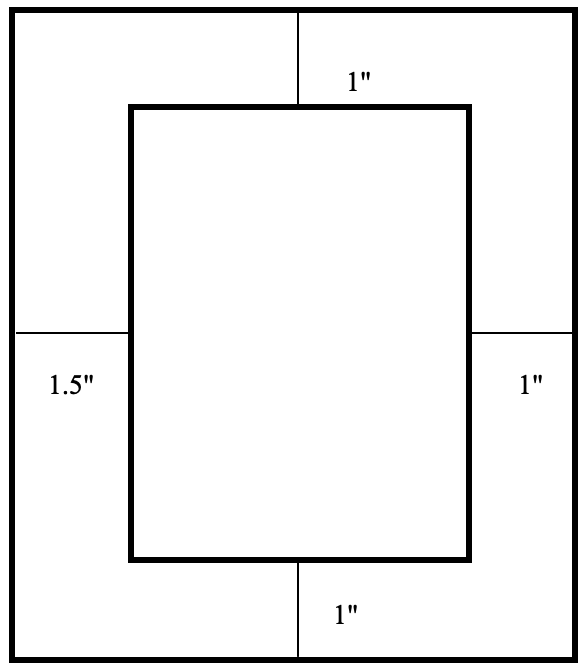
\includegraphics[width=110mm,scale=0.6]{page-padding.png}
        \caption{การเว้นระยะห่างจากริมกระดาษ}
        \label{fig:page-padding}
    \end{figure}

\subsection{เลขที่หน้า}

\begin{enumerate}
    \item ตั้งแต่บทคัดย่อถึงสารบัญ ให้ใช้ตัวอักษรโรมัน I, II, III, IV, … แสดงเลขหน้า โดยพิมพ์ไว้ตรงกลางส่วนล่างของหน้า ห่างจากด้านล่าง 1 นิ้ว
    \item ในส่วนของเนื้อหา (บทที่ 1เป็นต้นไป) ให้ใช้ตัวเลขอารบิค 1, 2, 3, 4, … แสดงเลขหน้า โดยพิมพ์ไว้ด้านขวามือห่างจากขอบบน 0.5 นิ้ว และห่างจากริมขอบกระดาษด้านขวามือ 1 นิ้ว หน้าแรกของแต่ละบทไม่ต้องมีเลขหน้าปรากฏ แต่นับรวมเป็น 1 หน้า
\end{enumerate}

\subsection{การพิมพ์ตาราง}

ให้แทรกปนไปในแต่ละบทของเนื้อเรื่องที่มีความสัมพันธ์ โดยพิมพ์"ตารางที่"อยู่ด้านบน (ใช้อักษร ตัวหนา) ชิดขอบซ้ายของหน้ากระดาษ ตามด้วยชื่อตาราง (ใช้ตัวอักษรปกติ) ถ้าชื่อตารางมีความยาวเกินกว่า 1 บรรทัด ให้พิมพ์บรรทัดล่าง เริ่มพิมพ์ตรงกับตัวอักษรตัวแรกของคำบรรยายตาราง พิมพ์ตารางโดยไม่ต้องเว้นบรรทัดจากชื่อตาราง เมื่อพิมพ์ตารางจบแล้วให้เว้นไว้ 1บรรทัดก่อนการพิมพ์ปกติหากตารางไม่จบในหน้าเดียวให้ขึ้นหน้าใหม่ โดยพิมพ์คำว่า ตารางที่ ........ (ต่อ) แล้วตามด้วยชื่อตาราง

\subsection{การเรียงเลขตาราง}

ให้เรียงไปตามบท เช่น ในบทที่ 1 ให้พิมพ์ตารางที่ 1.1, ตารางที่ 1.2 ในบทที่ 2 ให้พิมพ์ ตารางที่ 2.1, ตารางที่ 2.2 เป็นต้น

\subsection{การพิมพ์รูป}

ให้เว้น 1 บรรทัดก่อนจัดวางรูปภาพกลางหน้ากระดาษ และใส่คำว่า "รูปที่……" โดยใช้ตัวอักษร ตัวหนา ตามด้วยคำบรรยายไว้กึ่งกลาง ใต้ภาพ ถ้าคำบรรยายเกิน 1บรรทัดให้พิมพ์บรรทัดล่างเริ่มพิมพ์ตรงกับอักษรตัวแรกของคำบรรยายภาพ และเว้น 1 บรรทัด ก่อนพิมพ์ปกติต่อไป การเรียงหมายเลขรูปที่ ให้เรียงไปตามบทเช่นในบทที่ 1 ให้พิมพ์รูปที่ 1.1, รูปที่ 1.2 ในบทที่ 1 ให้พิมพ์ รูปที่ 2.1, รูปที่ 2.2 เป็นต้น

\subsection{การพิมพ์เครื่องหมายวรรคตอน}
\begin{itemize}
    \item เครื่องหมายมหัพภาค	(.) 	ให้พิมพ์	เว้นระยะ 	2 อักษร
    \item เครื่องหมายจุลภาค	(,)	ให้พิมพ์เว้นระยะ 	1 ช่วงตัวอักษร
    \item เครื่องหมายอัฒภาค	(;)	ให้พิมพ์เว้นระยะ 	1 ช่วงตัวอักษร
    \item เครื่องหมายมหัพภาคคู่	(:)	ให้พิมพ์เว้นระยะ	1 ช่วงตัวอักษร
    \item เครื่องหมายอัญประกาศ	(“  ”)ให้พิมพ์เว้นระยะ 		1 ช่วงตัวอักษร
\end{itemize}


\subsection{การเขียนบรรณานุกรม}

เป็นส่วนที่แสดงถึงการศึกษาค้นคว้าวิจัยของผู้เขียนว่า มีความสมบูรณ์กว้างขวาง ลึกซึ้ง ทันสมัยน่าเชื่อถือมากน้อยเพียงใด โดยทั่วไป คำว่า บรรณานุกรม รวบรวมรายการเอกสารสิ่งพิมพ์ โสตทัศน์ สื่ออิเล็กทรอนิกส์ ที่ผู้เขียนศึกษาค้นคว้าทั้งหมด แม้ว่าจะไม่ได้คัดลอกข้อความมา ส่วนคำว่า เอกสารอ้างอิงนิยมใช้กับรายการเอกสาร สิ่งพิมพ์ โสตทัศน์ เฉพาะที่คัดลอกและยกมาอ้างอิงในเนื้อหา
บรรณานุกรมเป็นส่วนประกอบสำคัญส่วนหนึ่งของการผลิตสิ่งพิมพ์โดยเฉพาะสิ่งพิมพ์ประเภทตำราหรือหนังสือเรียน และเอกสารประกอบการสอน เพราะเป็นส่วนที่ระบุถึงหนังสือและเอกสารต่าง ๆ ตลอดจนการสัมภาษณ์ที่ผู้เขียนใช้เป็นแหล่งข้อมูลในการอ้างอิง

\textbf{ตัวอย่างการแทรกบรรณานุกรมที่อ้างอิงถึง}

เนื่องจากในการถอดรหัสในเชิงความถี่นี้จะต้องใช้การแปลงและแปลงกลับเป็นส่วนสำคัญ \cite{schroffFaceNetUnifiedEmbedding2015} นอกเหนือไปจากการคำนวณอื่นๆ การแปลงและการแปลงกลับจะต้องใช้การคำนวณเป็นจำนวนมากจึงมีการนำวิธีการตัวประกอบปฐม (Prime factor Algorithm) มาใช้เพื่อลดจำนวนการคำนวณลงโดยใช้ร่วมกับวิธีการแปลงข้อมูลจำนวนน้อยๆ (Short Length Algorithm) \cite{sagonas300FacesIntheWild2013} ในแง่ของการนำวิธีการดังกล่าวไปใช้งานจริงซึ่งจะต้องพิจารณา
